\documentclass[a4paper,12pt]{article}
\usepackage[utf8]{inputenc}
\usepackage[english]{babel}
\usepackage[T1]{fontenc}
\usepackage{minted}
\usepackage{adigraph}
\usepackage{graphicx}
\usepackage{cite}
\usepackage{url}
\usepackage[colorlinks,pdfpagelabels,pdfstartview = FitH,bookmarksopen = true,
bookmarksnumbered = true,linkcolor = black,plainpages = false,hypertexnames = false,
citecolor = black] {hyperref}

\pdfbookmark[1]{tableofcontents}{toc}
\title{Snake-AI\\Project Documentation}
\author{
		Ibrahim Enes Hayber, Rana MD Jewel, Maximilian Lüttich\\
		Frankfurt University of Applied Sciences\\
		Faculty 2, Computer Science (B. Sc.)\\
		Object-oriented Programming in Java by Prof. Dr. Doina Logofatu
}

\date{\today}

\begin{document}

\maketitle
\begin{center}

\includegraphics[scale=0.8]{fra-uas-logo}
\end{center}
\newpage
\tableofcontents

\newpage
\section{How we started}
In this chapter we will briefly describe how we started working on the task that we had chosen after the first part of the Java-course was completed.\\
\\As we all know, the hardest part of any task is getting started. But once the start has been made, the later steps seem to follow naturally.
You could think of this as  a series of dominoes that all fall after the first one has been knocked over.\\
\\As usual with any task, first one needs to precisely understand what the problem is and what are the requirements to solve the problem. In order to do just that, we carefully read the description of the organizers and in addition to that, we watched a few videos on our topic.\\
\\After each team member became familiar with the task, we started working with the Snake AI framework, which was provided in a GitHub repository. The framework was written in the Java programming language. If anything was unclear, we used the UML class diagram to get a better understanding of the structure of the problem. We also watched an extensive YouTube tutorial, also provided by the organizers, that enabled us to quickly create our first bots. In the following chapters, a detailed introduction and our results will be presented.
\newpage

\section{Introduction}
Many are familiar with the game “Snake”, which became famous because it was preinstalled on a popular Nokia device back in 1997.\cite{nokia}
However, the essence of our project was to look at this game from a slightly different perspective. 
What made our task special was that instead of manually moving a single snake, we were to create two intelligent snake bots competing against each other.
The goal of a bot is to win, following the rules that will be described later on.
This chapter focuses on the general overview of this project and comparison with similar problems in practice.
\subsection{General Topic}
As already mentioned, our main task was to create snake bots that had to be as intelligent as possible. To create such bot, all we had to do was to implement a class that implements the Bot interface. This interface has only one method, which is the \textit{chooseDirection()} method. One could say that this method simulates the brain of the bot. The return value of this method is the direction in which the snake should move. As possible directions we have \textit{up, down, left or right}.For example, a bot could be implemented that turns right every time. But such a bot would of course be very uninteresting. For our project, we wanted to create bots that use artificial intelligence algorithms or other complex structures. \\ \\First of all, the rules of the game are presented below.\\
\\
\textbf{Rule 1:}  A bot controls only the direction (going either north, south, east, or west) to
be taken by its own snake.\\
\textbf{Rule 2:} Snakes always move simultaneously and forward. Their size increases by one position
(i.e. pixel) after taking an apple.\\
\textbf{Rule 3:} A Snake loses in any of these conditions:\\
\begin{enumerate}
\item If it leaves the board;
\item If it hits its own body;
\item If it hits the other snake's body;
\item If it takes more than one second to make a decision (i.e. which direction to take).
\end{enumerate}
\textbf{Rule 4:} If snakes collide head to head, the longest snake wins the game.\\
\textbf{Rule 5:} Apples appear randomly at an unoccupied position of the board, and there is only
one apple available at any time.\\
\textbf{Rule 6:} An apple will disappear if it is not eaten by either snake in 10 seconds and reappear
somewhere else on the map.\\
\textbf{Rule 7:} At the end of the tournament, players are ranked according to the number of
victories; then the number of draws; then the result of\\

\subsection{Similar problems in practice}
Since the bots did not have an easy task to solve, it was necessary to use smart solution methods to produce a favorable return value for any given position of the game. What if we could implement a bot that just roughly goes after the apple. Would this be enough to call it a smart bot? Of course not. It is in principle a desired behavior of our snake to reach for apples, but that is generally not enough. It should also take the shortest path to the apple. For example the Dijkstra algorithm can be used to get a such a shortest distance. The Dijkstra algorithm is a graph based algorithm which calculates the shortest path from one node to every other node. To get a better understanding of this concept, we will give an example below.\\
\\
\begin{figure}[H]
\centering
\NewAdigraph{mygraph}
{
A,blue:0,0;
B:2,0;
C:2,2;
D:0,2;
E,blue:1,3.4
}
{
A,B:12;
B,C:4;
C,A:7; 
A,D, red :1;
D,E, red :2; 
E,C:5;
C,D:9;
}[-]
\mygraph{}
\caption{Dijkstra Graph Example}
\end{figure}
In the given example we want to know the shortest path from node A to node B. A human can easily look at the graph and see that taking the route from A-D at the cost of 1 is much better than taking A-C at the cost of 7, or A-B at the cost of 12. Next, we would also see that we have a cost of 2 from D-E. In total we see that the shortest path from A to D is A-D-E. Since a computer cannot "see" the cost of each edge the concept of simply looking at the graph is not an option for it. That is why we have algorithms like Dijkstra, which calculate and erase paths with higher costs and return to us the shortest path.\\
\\There are many everyday problems where we are using algorithms to compute the shortest path. Using a navigation tool to drive from one city to an other city is one example of such a usage. We all would be in serious trouble, if a navigation tool would take any random path to a destination rather than taking the shortest path, or the path with lowest travel time.\\
\\This is of course not the only use case of Dijkstra in real life applications. When we talk about computer networks, we will also find the use of Dijkstra, considering IP-routing to find the shortest path between the source and the destination router. Dijkstra algorithm is commonly used in routing protocols for updating the forwarding tables.\\
\\In a scenario, where robots are used, you surely want them to work efficiently. Drones and robots, which are working automatically, are using pathing algorithms.\\
\\Even many dating or social media applications are using Dijkstra to recommend a user to another user. The users are seen as nodes. The distance could be defined by different parameters like common friends, same interests or even living in the same city.\cite{geeksdijkstra}\\
\\A fascinating real life application would be using algorithms to make emergency calls more efficient. Based on the location of the caller, the algorithm calculates, for example, which firefighter department is the closest one. Of course, the same concept could be used for calling police departments and hospitals.

\section{Team Work}
The project "Snakes AI" offered many possibilities to try out different approaches regarding team
work. Separate parts of this project were tackled by us using a way of working that seemed
appropriate for this segment. Our way of working only became apparent during the course of the
project and was not determined by us from the outset. Now, in retrospect, some thoughts on
teamwork will be discussed in the following.\\
\\In order to understand the given problem in detail, we frequently met virtually on a Discord server,
which we had already created for the first part of the Java-Class, that consisted mainly of solving
Kattis tasks. Furthermore, we initially embraced the opportunity to ask questions during the OOP-
exercises at the university. Our tutors, Mrs. Garbaruk and Mr. Mim, were usually able to help us
very quickly and sometimes gave helpful hints on the further development of our project.\\
\\The meetings on the Discord server were maintained by us at regular intervals until the completion
of the project. Discord offers many useful features that simplify team work. Chat rooms, data
transfers, screen sharing, and meeting rooms are some of the benefits of this program, that
eliminated the need for physical team meetings aside from our weekly meetings at the OOP-
exercise.\\
\\After the initial comprehension questions had been clarified, the work on the creation of bots began.
Initially, each team member had started working independently of the other team members on their
own design of a bot. At this point, communication within the team was secondary, each team
member tried to create their own bot. In retrospect, this approach turned out to be beneficial, since it
gave us the opportunity to test different designs with different strengths and weaknesses.\\
\\After the first executable results were available, we began to present them to each other and had
them compete against other bots that were available. In doing so, we tried to identify weak points
and to work together cooperatively on promising ideas.\\
\\By this point of the development, we also started using Github, which made a lot of things easier for
us. For example we used Github to maintain different versions of our project. Using Github was for all of us a new experience. We also faced some problems in the beginning where we could not merge our project. As Team we fixed this problems. One of them was that two persons changed something in the same line. So communicating was key to success.\\
\\Since each team member was very motivated, we were able to do both - continue working
individually on a bot and maintain a supportive exchange during the meetings. A friendly
competition served each member as an incentive to further develop their own bot. We think that the
combination of individually working on a project and afterwards discussing the results in a team
meeting has turned out to be a very effective way of creating and improving bots. Even though we
tried to initiate a competition, the communication among the team members was always friendly
and solution-oriented.\\
\\Even if the original idea of every bot can be traced back to a single team member, we will always
use "we" at the appropriate point in the documentation. Because every team member contributed
something to every bot during the various stages of development.
\newpage	

\section{Problem Description}
As already mentioned in the second part of this documentation "Introduction",
our task was to create and evaluate bots for the well-known game "Snake".\\
\\What was special about this project was that we were provided with a functioning graphical user interface.
This also included an extensive library of classes with corresponding functions, a "bot" interface, an enumeration, 
and also some sample bots. On the one hand, this allowed us to concentrate exclusively on working on bots,
but on the other hand, it was a challenge to get a precise understanding of the task at the beginning.
An overview of all given things shall be given in chapter 7 - "Implementation Details" - of this documentation.\\
\\The game "Snake" consists of a rectangular game board on which two snakes move around.
The board  is divided into small squares of equal size.
A snake consists of a head and several body elements. 
The head and each body element completely fills out exactly one such square.
A movement of the snake is performed starting from the head.
All elements of the body and the head perform a movement at the same time. 
A snake never moves diagonally and only ever makes one of the following moves: up, 
down, right, left. One movement consists of the $(n+1)$th element of the snakes body 
taking the position of the nth element of the body etc. The $0$th element is the head of the snake.
\\
\begin{figure}[h]
    \centering
    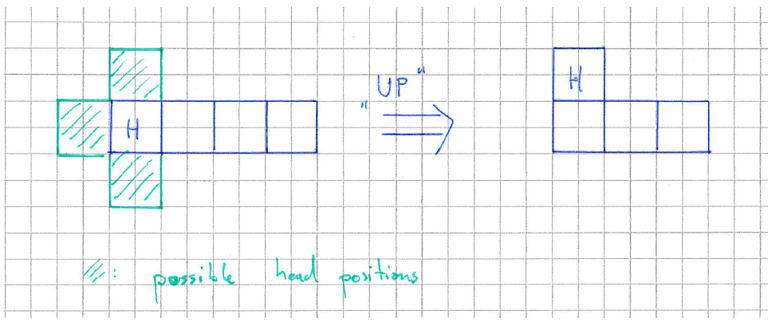
\includegraphics[scale=0.8]{snakeForward.png}
    \caption{Snake movement}
    %\label{fig:abc}
\end{figure}
\newpage The two snakes competing against each other perform their movements simultaneously. 
Furthermore, one square of the game board represents an apple. 
If a snake's head moves onto the square representing an apple, the apple disappears,
a new apple appears at a random location, and a new body element is appended to the already existing body elements. 
The new element occupies the square from which the snake's body would have just moved away. If the apple has not been reached 
after ten movements, it disappears and a new apple is created at the same time in a different place. The exact rules of when
a snake loses or wins have already been presented in Section 2.1.  . All parameters, such as the size of the game board,
starting points of the snakes, and the number of rounds, can be adjusted in the methods of the SnakesUIMain class.
 \begin{figure}[h]
    \centering
    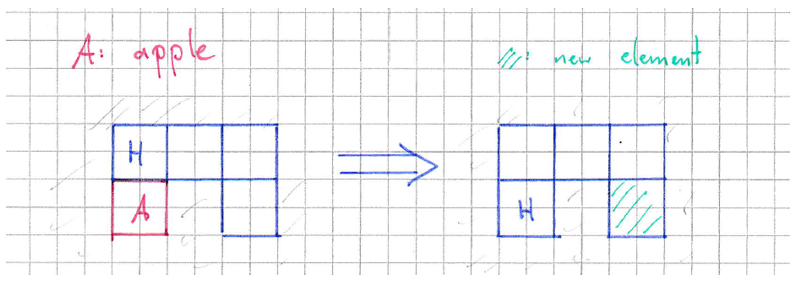
\includegraphics[scale=0.8]{SnakeApple.png}
    \caption{Snake Apple}
    %\label{fig:abc}
\end{figure}
A bot can be easily created by implementing the given interface "Bot". This interface contains a single function 
"chooseDirection" that needs to be overridden in a bot class to create a valid bot. The function has four parameters:
"Snake snake", "Snake opponent", "Coordinate mazeSize" , "Coordinate apple". "Snake" and "Coordinate" are already given 
classes. As a return value, this function has to provide a direction in which the snake's head should move in the next round.
The value of a direction is realized by the enum "Direction".\\
\\The individual squares of the game board are represented by objects of the 
"Coordinate" class, which implements the "Comparable" interface. An object of the
"Coordinate" class consists of two integer values, the x and the y component, a constructor 
and several useful methods. A very important object of this class is "mazeSize". This object 
contains the least upper bounds for the x and y values of the coordinates of the game board and 
is used, for example, to decide whether another “Coordinate”-object is inside or outside the game board.
It is initialized inside the SnakesUIMain class. Two parameters of this type are passed to 
the "chooseDirection" function - the coordinate of the apple and the already mentioned "mazeSize" object.\\
\\A snake of this game is described by an object of the "Snake" class. An object of the class "Snake"
consists of a HashSet "elements" whose elements are objects of the type "Coordinate", a deque "body"
whose elements are also objects of the type "Coordinate" and a "Coordinate" object "mazeSize", which 
should be initialized with the least upper bounds for the x and y values of the coordinates of the game
board. Various constructors and useful methods are also implemented in this class. "elements" and "body" 
of a "Snake" object contain the same values for different uses. Two parameters of this type are passed to 
the "chooseDirection" function - "Snake snake", the snake for which a direction has to be found and "Snake opponent", the opposing snake.\\
\\Based on these four parameters alone, an advantageous direction for the snake controlled by the bot 
must be found. This direction is then passed as a return value in the form of an enum "Direction" value. 
There are naturally four choices within this enumeration: Direction.UP, Direction.DOWN, Direction.LEFT,
Direction.RIGHT. These can be interpreted as directional vectors constrained to an adjacent coordinate.\\
\\A comprehensive tutorial on how to create a simple bot was also available to us on the follwing website: 
https://github.com/BeLuckyDaf/snakes-game-tutorial. We used this tutorial excessively at the first, but then 
gradually moved on and tried out our own ideas.

\section{Related Work}

In recent years, the development of artificial intelligence algorithms has seen a rapid growth,
and this growth has been particularly evident in the field of gaming. Snake, as a classic and popular game, 
has been a subject of research in the field of AI and has attracted a great deal of attention from researchers.\\
Several studies have focused on developing AI algorithms for playing Snake. For instance, reinforcement learning 
algorithms have been used to train AI agents to play Snake and improve their gameplay. Genetic algorithms have also
been applied in this context, enabling the evolution of AI agents to play Snake at a high level.\\
There has also been work on developing multi-agent systems for Snake, where multiple AI agents compete against each other.
This approach has been used to explore topics such as collaboration and competition in AI systems, as well as the development of more advanced AI algorithms.\\
There are also some other Games that implement the same Algorithm as Snake AI.\cite{RelatedWork}
\begin{itemize}
\item Flappy Bird AI
\item Breakout AI
\item Tetris AI
\item PacMan AI
\item Mario AI
\end{itemize}
For instance,Mario AI games use artificial intelligence techniques to control the actions of the character,
Mario. This can be done through techniques such as reinforcement learning, evolutionary algorithms,
or rule-based systems. The AI system receives inputs from the game environment and based on these inputs,
the AI model outputs actions for the player character, such as jumping, running and shooting.
The AI's goal is to complete the game's objectives while avoiding obstacles and enemies.
The performance of the AI is often evaluated based on metrics such as completion time, number of lives lost, and score.

\section{Implementation Details}
\subsection{Application Structure}
The Snake AI game consists of a interface, several classes and an enumeration, including: 
\begin{itemize}
\item Bot(Interface)
\item Direction(Enum)
\item BotLoader
\item Coordinate
\item Snake
\item SnakeGame
\item SnakeCanvas
\item SnakesRunner
\item SnakeUIMain
\item SnakesWindow
\end{itemize}

\subsection{GUI Details}
In this section, comprehensive details of all classes will be thoroughly discussed.
\subsubsection{SnakeUIMain}
This class serves as the starting point for the Snake game tournament, where several rounds of the game are conducted.
The main method of the class accepts two instances of the class Snake (snake and opponent) as arguments.\\
It is responsible for initiating rounds of the Snake game between the bots, managing I/O operations such as recording the score of the opponent and snake,
apples consumed by both snakes, and the time taken in each round. These records will be used for future statistical analysis.
\subsubsection{BotLoader}
The BoatLoader class retrieves the specified class based on its name and package from the classpath.
It enables the dynamic addition of classes to the Bot game after it has been initiated. This class inherits the abstract Java ClassLoader class.\\
A class loader is an object that is responsible for loading classes.ClassLoader is an abstract class.
When the name of a class given, a class loader should attempt to locate or generate data that constitutes a definition for the class. 
A typical strategy is to transform the name into a file name and then read a "class file" of that name from a file system.\cite{classLoader}
The only method of BotLoader class gets classBinName as argument and returns an instance of the Bot class.

\subsubsection{SnakesWindow}
The SnakesWindow class manages the graphical user interface of the game. It creates and sets up the window, runs the UI, and closes the frame when necessary. This class implements the Runnable interface.
The Runnable interface is intended for classes whose instances are meant to be executed by a thread. 
It requires the implementation of a method called 'run' that takes no arguments. The interface provides a standard protocol for objects that need to run code while active. For instance, the Thread class implements Runnable.
Being active refers to a state where a thread has been started and is yet to be stopped.\\
Moreover, Runnable allows a class to be active without requiring it to subclass Thread. A class that implements Runnable can run without subclassing Thread by instantiating a 
Thread instance and passing itself in as the target. In most cases, the Runnable interface should be used if you are only planning to override the run() method and no other Thread methods. This is important because classes should not be subclassed unless the programmer intends on modifying or enhancing the fundamental behavior of the class.\cite{runnable}
\subsubsection{SnakesRunner}
This class also implements Runnable interface and is used for running bots in a separate threads.
The Constructor of the class SnakesRunner gets running bot, snake that is controlled by the current bot,
opponent's snake, size of the board and coordinate of current position of the apple as arguments.
In addition, the chooseDirection method of the current bot is executed and saved(current direction) by this class. 
\subsubsection{SnakesGame}
The SnakesGame class implements the central gameplay flow and executes the game for two bots.
It overrides the toString() method to convert the game into a string representation and return the current game state as a string.
The randomNonOccupiedCell() method selects a random cell in the maze that is not occupied, which is used to generate a new location for the apple.
Additionally, the runOneStep() method terminates the current round if a snake takes more than one second to choose its next direction.

\subsubsection{SnakeCanvas}
The SnakeCanvas class designs the graphical user interface and enhances its appearance. It is responsible for coloring the body of the snake and opponent, making them visible on the UI.
The render() method renders the game window after filling the body of the snake, opponent and apple.
With each movement of the snake, opponent, and apple, the previously occupied positions are re-colored and marked as available for further movements.
This class inherits the Java Swing class JPanel, which is used to create various lightweight containers that can hold one or more components.
\subsubsection{Snake}
The Snake class implements the physical representation of the snakes on the game board, determining the position of snake's head, body, and length.
To achieve this, the class utilizes two efficient and logical data structures from the Java Collections framework. Each of them contains the Objects of the class "Coordinate" as elements. They are,
\begin{itemize}
\item Dequeue
\item HashSet
\end{itemize}
Those two structures contain same values, but for different purposes.
The Deque (double-ended queue) data structure allows the addition and deletion of elements from both the ends(head and tail) in $\mathcal{O}(1)$ time complexity. 
The HashSet data structure ensures basic searching, addition and deletion operations in $\mathcal{O}(1)$ time complexity .\\
This class has a important feature of cloneability which allows to copy one Object to another object without using new operator.
A class implements the Cloneable interface to indicate to the Object.clone() method that it is legal for that method to make a field-for-field copy of instances of that class.
Invoking Object's clone method on an instance that does not implement the Cloneable interface results in the exception CloneNotSupportedException being thrown.\cite{Cloneable}
\subsubsection{Coordinate}
The Coordinate class implements the position of a cell on the game board. It helps in the growth of the snake body by adding a new coordinate at the beginning of its body.
The inBounds() method ensures that the snake stays within the boundaries of the game board. This method implements the Comparable interface, making it useful in comparing two Coordinates. 
\subsubsection{Bot}
To create a working bot, all we have to do is to generate a class that implements the “Bot”-interface
The Bot interface defines a single method, chooseDirection(), which represents the decision-making process of the bot.
This method returns the direction in which the snake should move, with the options being up, down, left, or right.
\subsubsection{Apple}
Apple is an instance of the class "Coordinate".
\subsection{UML Diagram}

\begin{figure}[h]
\centering
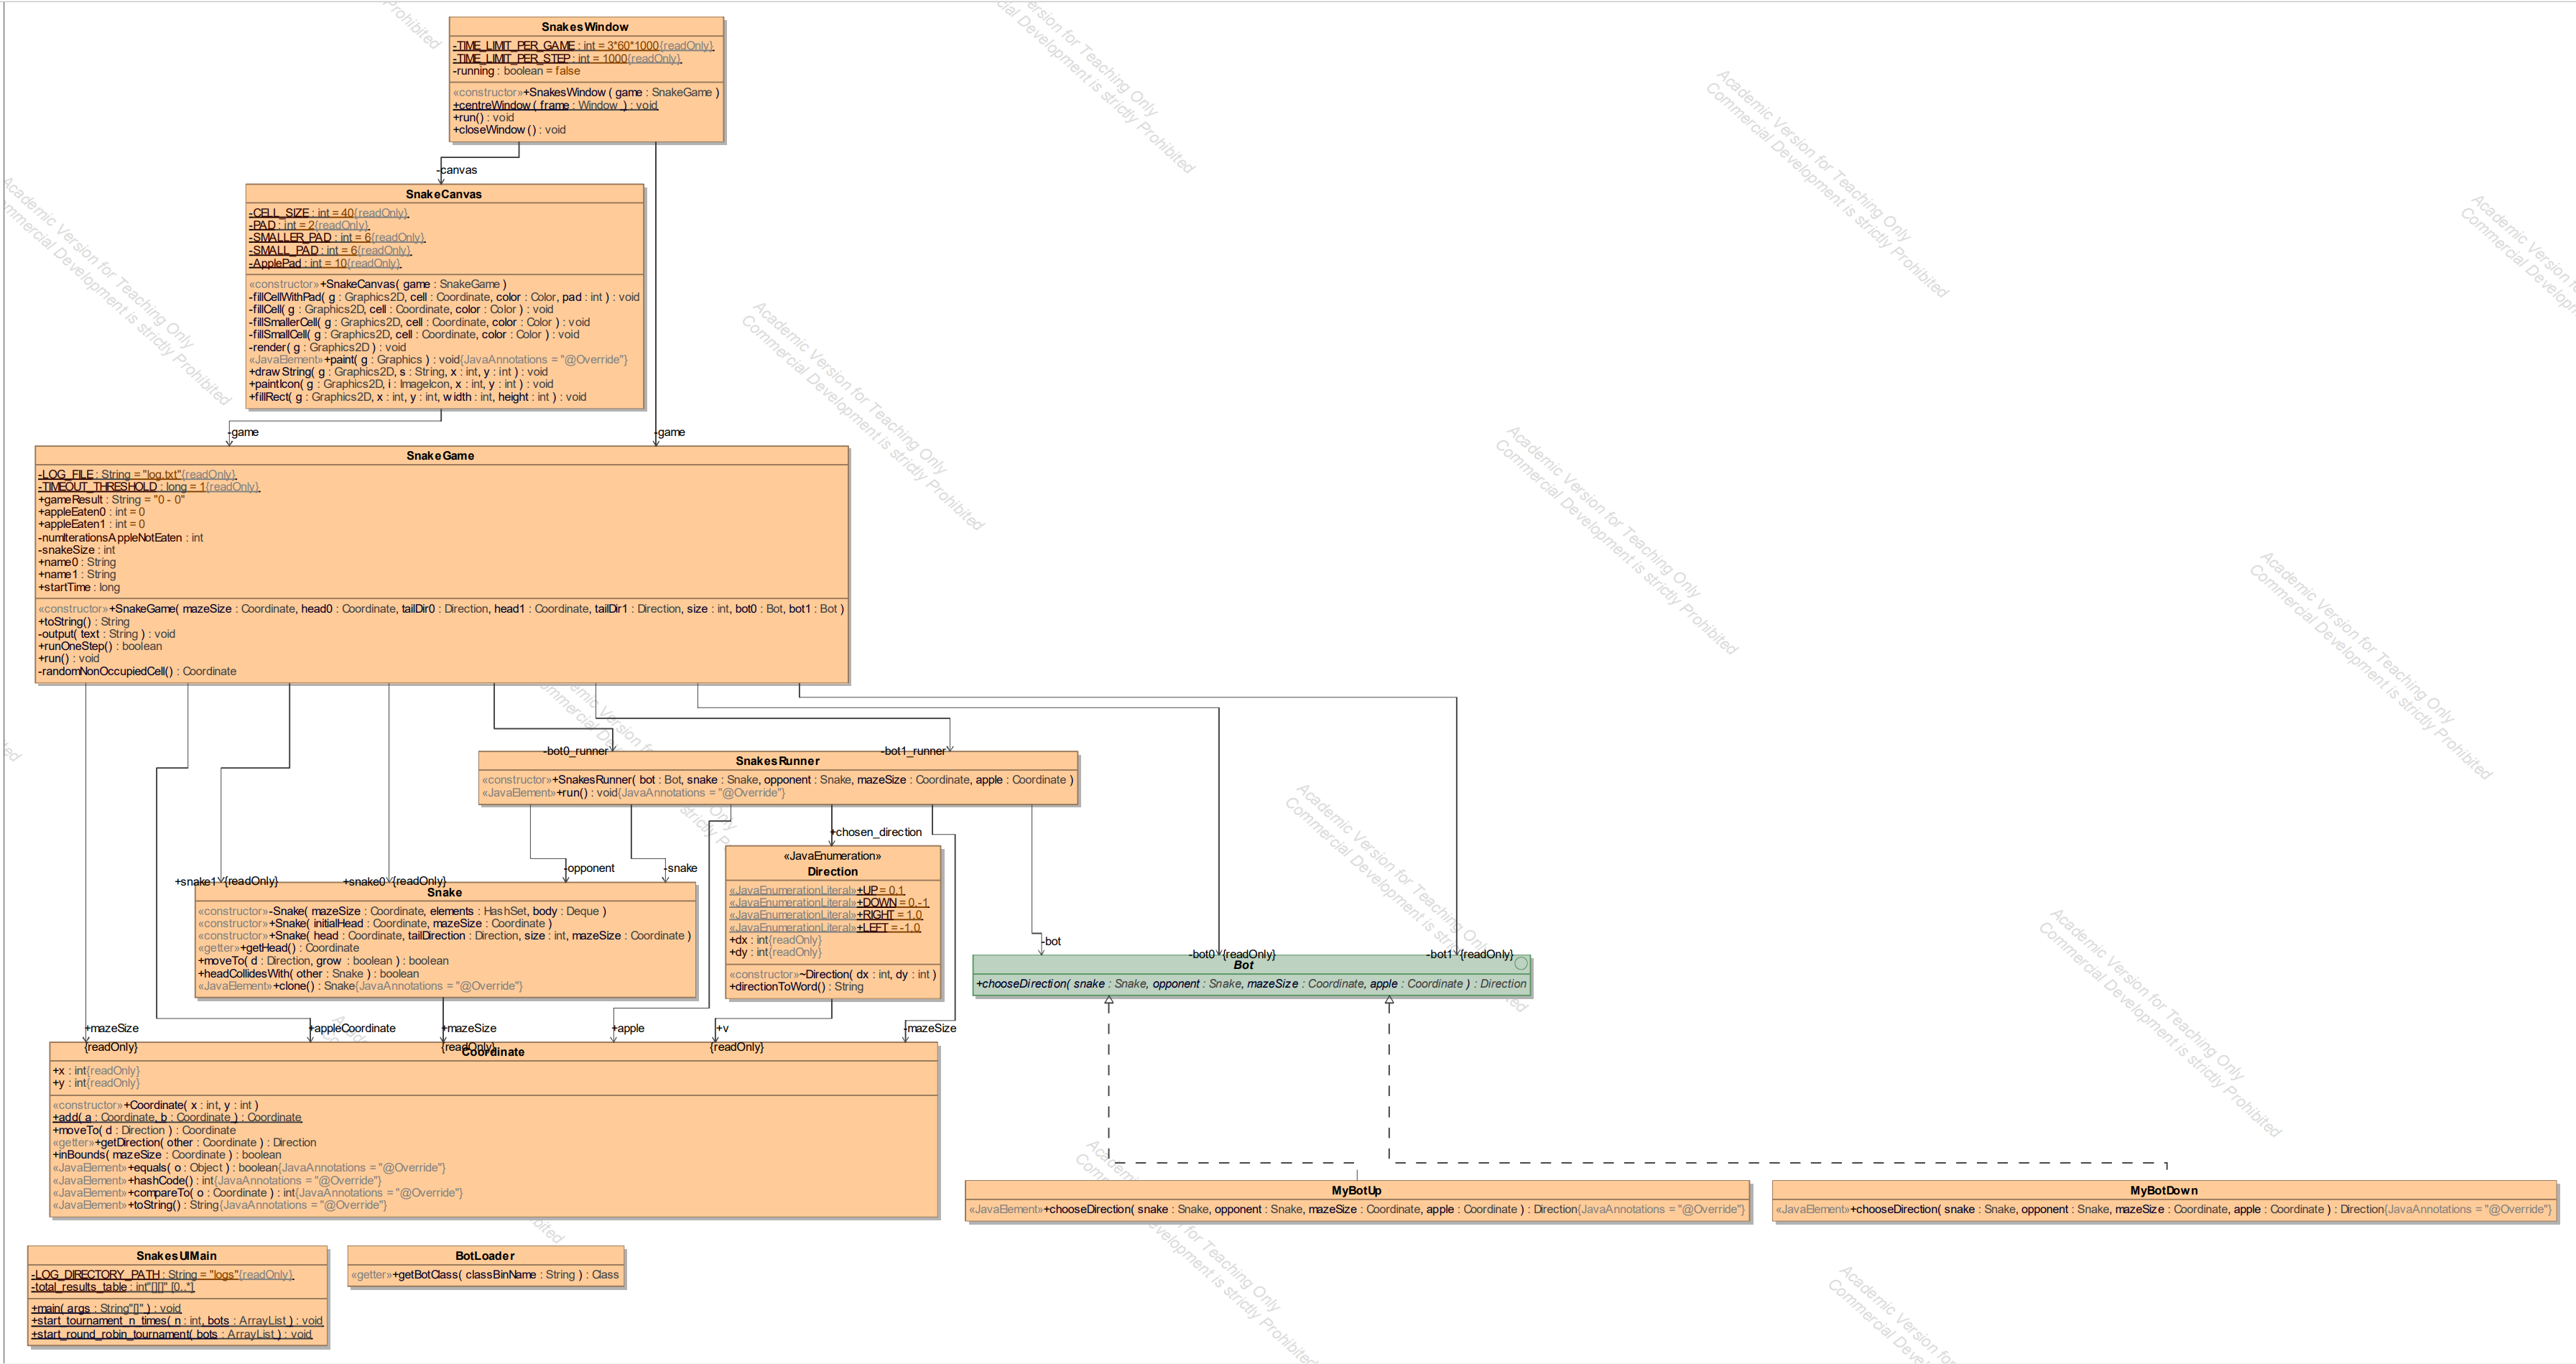
\includegraphics[scale=0.26]{ui.png}
\caption{UML diagram of the GUI}
%\label{fig:abc}
\end{figure}

\subsection{Used Libraries}
For the Developement of the Snake AI Game Java Swing Framework has been used.
Some Components from AWT framework have also been used.\\ 
Swing is a Java Foundation Classes [JFC] library and an extension of the Abstract Window Toolkit [AWT].
Swing offers much-improved functionality over AWT, new components, expanded components features, and excellent event handling with drag-and-drop support.\cite{awt}

%\subsection{Code Snippets} write code snippet with discription.
\section{Our Bots with different implementations}
\subsection{Bot1}
\subsubsection{IntBot1}
After getting to know the framework of our task, one of our first objectives was implementing a
basic bot by ourselves that does the following:\\
\begin{itemize}
\item Calculate all valid moves
\item Exhibit a basic avoidance behavior regarding the opponent
\item Go for the apple
\end{itemize}
This basic bot also served as an opponent for more advanced bots later on.\\
\\
To keep things organized, we decided to create a package for each bot. The packages were created
in the „src“-folder of the given project. Each bot consists of a public class that implements the
Interface „Bot“, which as previously described, consists of only one method: „chooseDirection“.
Properly overriding this method turned this class into a bot that could be used in the game.
\\
\\
The basic idea for creating this bot was that a static array that contains all possible directions
(Direction.RIGHT, Direction.DOWN, Direction.UP, Direction.LEFT) is created outside the method
„chooseDirection“ and inside the method each element of this array is checked for its worth
concerning the stated objectives. This concept was also used in the provided example of  a bot  on the following website: \url{https://github.com/BeLuckyDaf/snakes-game-tutorial} The only thing that this bot was concerned with was not killing itself.\\
\\
Creating the static array:
\begin{minted}{java}
public class IntBot1 implements Bot {
private static final Direction[] DIRECTIONS = new Direction[]{Direction.RIGHT,
Direction.DOWN, Direction.UP, Direction.LEFT};
@Override
public Direction chooseDirection(Snake snake, Snake opponent, Coordinate
mazeSize, Coordinate apple) {
\end{minted}
The first thing we did was to create an array of possible directions of the opponent’s head and a set
that contains the resulting coordinates, so that at the end of the method „chooseDirection“ the
coordinates could be removed from the pool of possible directions of our bot’s head. To create such
an array, it was necessary to determine the coordinate of the second element of the opponent snake.
We used an iterator to achieve this in the following way:\\
\begin{minted}{java}
//Position of second Element of opponent
Coordinate afterHeadNotFinal2 = null;
if(opponent.body.size()>=2){
Iterator<Coordinate> it = opponent.body.iterator();
it.next();
afterHeadNotFinal2 = it.next();
}
final Coordinate afterHead2 = afterHeadNotFinal2;
//second element of opponent snake
\end{minted}
Note that the class „Snake“ featured a deque of elements of the „Coordinate“-class called „body“.\\
\\
After that, we used a stream method to get a sequential stream of the elements from the array
„DIRECTIONS“ to create a new array of directions called „validMovesOpponent“. The direction
whose result would equal the second element of the opponent snake was filtered out using the “equals”-method on coordinate objects. Finally, a Set of coordinates called
“possiblePositionsOpponent” was created by simply using the “moveTo” method on the head of the
opponent snake and having all elements of “validMovesOpponent” as parameters.
\begin{minted}{java}
Direction[] validMovesOpponent = Arrays.stream(DIRECTIONS)
.filter(d -> !head2.moveTo(d).equals(afterHead2))
.sorted()
.toArray(Direction[]::new);
Set<Coordinate> possiblePositionsOpponent = new HashSet<>();
for(int i=0; i< validMovesOpponent.length; i++){
possiblePositionsOpponent.add(head2.moveTo(validMovesOpponent[i]));
}
\end{minted}


Since no other restrictions were made, the set „possiblePositionsOpponent“ always contained three
elements, even if they were to be outside the maze.\\
\\
Analogous to the array „validMovesOpponent“ we created an array of directions called
„validMoves“ for our bot’s snake that excluded the possibility of backwards movement of the
snake. This array „validMoves“ was subsequently used as a parameter of the stream method to
create a new array of directions called „notLosing“, that with the use of the filter method excluded
some unfavorable outcomes.
\begin{minted}{java}
Direction[] notLosing = Arrays.stream(validMoves)
.filter(d -> head.moveTo(d).inBounds(mazeSize))
.filter(d -> !opponent.elements.contains(head.moveTo(d)))
.filter(d -> !snake.elements.contains(head.moveTo(d)))
.filter(d -> !possiblePositionsOpponent.contains(head.moveTo(d)))
.sorted()
.toArray(Direction[]::new);
\end{minted}

Using the filter method, we checked the following: Is the resulting coordinate outside the
maze? Is the resulting coordinate part of the opponent’s body? Is the resulting coordinate
part of our snake’s body? And finally, does the set „possiblePositionsOpponent“ contain the
resulting coordinate? If the answer to each of these question was „no“ the streamed element
was added to the array.\\
\\
Finally, we used the bubble sort algorithm to sort the elements of „notLosing“ based upon
the distance to the apple. „chooseDirection“ returns the first element of „notLosing“
provided that this array is not empty. If this array happens to be empty, the first element of
„validMoves“ is returned which, is never empty.
\begin{minted}{java}
//Bubble Sort; Sorting Elements of "NotLosing"
double distance1, distance2;
int a1, a2, h11, h12, h21, h22, d1, d2;
Coordinate test1, test2;
Direction temp;
if (notLosing.length > 0){
a1=apple.x;
a2=apple.y;
for(int i=0; i< notLosing.length; i++){
for(int a= i+1; a< notLosing.length; a++){
test1 = head.moveTo(notLosing[i]);
test2 = head.moveTo(notLosing[a]);
h11= test1.x;
h12 = test1.y;
d1 = (h11-a1)*(h11-a1)+(h12-a2)*(h12-a2);
distance1=Math.sqrt((double)d1);
h21= test2.x;
h22 = test2.y;
d2 = (h21-a1)*(h21-a1)+(h22-a2)*(h22-a2);
distance2=Math.sqrt((double)d2);
if(distance2<distance1){
temp=notLosing[i];
notLosing[i]=notLosing[a];
notLosing[a]=temp;
}
}
}
return notLosing[0];
}
else{
return validMoves[0];
}
}
\end{minted}
The biggest drawback of this bot was the frequent entrapment with itself or the opponent's snake. 
Even though basic evasive movements were often enough to avoid losing the game, more complex dangers like a U-shape of the opponent's
snake or the bot’s snake could not be recognized by this bot. This becomes more apparent the more elements the bodies of the snakes have.
\subsubsection{RecursiveBot}
\label{RecursiveBot}
\textbf{Preliminary consideration:}\\
\\Since "IntBot1" turned out to be very vulnerable to self-entrapment or entrapment by the opponent,
we started to search for a solution to this specific problem. We conducted our search by overriding
IntBot1's "bubble sort" section with various other approaches. In order to subsequently evaluate the
different results, we had the resulting bots compete against one another several hundred times. This
quickly gave us a rough evaluation of a bots capabilities and showed us which idea was promising.\\
\\Our first idea consisted of an extension of the first part of "IntBot1" that creates more than one
possible enemy position. Several arrays were created containing these future moves of the
opponent. We were hoping that this would at least make our bot less prone to getting entrapped by
the opponent, but that wasn't the case. In the end, this bot turned out to be inferior to the original
"Intbot1", since many squares of the game board could no longer be accessed by it. The bot's
decisions led to defeat very quickly, since most of the time it returned a value from the
"validMoves" array, which, for example, led to our snake leaving the game board. As a reminder,
"validMoves" contained all possible moves, except for the backwards movement of the snake\\
\\Another idea was to save different constellations of the two snakes, the apple, and the already
precalculated best possible movement. Thus, the only task of the bot would be to recognize a
position and select an already calculated solution from a database. For example, comprehensive
databases for analyzed chess positions have already been created in this way. \cite{chesstable}
Here, however, the very large number of possible positions represented an insurmountable obstacle
for us, which is why we soon gave up this idea.\\
\\A recursive function for evaluating possible moves turned out to be a very neat solution to the
problem of self-entrapment. The basic idea was as follows. Starting from the snake's head, all four
surrounding fields are scanned using a recursive method. If there is a collision with the snake's own
body or with the opponent, a bad rating is returned. If the apple is reached, a good rating can be
returned. However, this should also depend on whether the snake still has free squares available
after reaching the apple. Reaching the apple and subsequent entrapment are of course undesirable!
If nothing special happens, a neutral rating should be returned. Starting from the simulated position,
the function then looks at the next possible set of squares. If not interrupted, this process is repeated
until the desired number of simulation steps has been reached - this is the final break condition of
the recursive function. Finally, the bot's ChooseDirection method returns the direction to the best
scoring square.\\
\\We created such a function by using various predefined methods of the “Snake” and “Coordinate”
classes. During the implementation, we realized that this function rendered much of the first part of
the bot "IntBot1" obsolete. For example, by checking all fields around the head, the second body
element of the snake is also always checked. Since this is counted as a collision, this coordinate
always gets the worst rating and is only called if the position of the snake is lost anyway. As a
result, we completely removed the first section of "IntBot1".\\
\\This resulted in "IntBot1" and "RecursiveBot" no longer having any identical lines of code, even
though "RecursiveBot" was developed directly from "IntBot1". In the following, "RecursiveBot"
will be presented in detail.\\
\\\textbf{ChooseDirection:}\\
\\In the following, the resulting "ChooseDirection" method of the bot "RecursiveBot" will be
analyzed first.
\begin{minted}{java}
public Direction chooseDirection(Snake snake, Snake opponent,
 Coordinate mazeSize, Coordinate apple) {
int simSteps=10;
Snake snake_left = snake.clone();
Snake snake_right = snake.clone();
Snake snake_up = snake.clone();
Snake snake_down = snake.clone();
...
\end{minted}
As already explained, the appropriate parameters are passed indirectly to the "chooseDirection"
method from the main function. These parameters serve as the basis for our decision-making
algorithm.
The first variable "simSteps" can in theory be chosen freely and serves as a termination condition
for the recursive function later on. (In our test runs, integers between 7 and 11 had proven to be
advantageous.) Then the "clone()" method of the "Snake" class is used to create four clones of the
object "snake", which contains all parameters of the snake that is controlled by the bot.
Subsequently these clones will be moved in the appropriate direction and evaluated.
\begin{minted}{java}
...
int val_left = Integer.MAX_VALUE;
if(snake_left.moveTo(Direction.LEFT, false)){
val_left= evaluateDirection(snake_left,opponent,apple,simSteps);
}
int val_right = Integer.MAX_VALUE;
if(snake_right.moveTo(Direction.RIGHT, false)){
val_right= evaluateDirection(snake_right,opponent,apple,simSteps);
}
int val_up = Integer.MAX_VALUE;
if(snake_up.moveTo(Direction.UP, false)){
val_up= evaluateDirection(snake_up,opponent,apple,simSteps);
}
int val_down = Integer.MAX_VALUE;
if(snake_down.moveTo(Direction.DOWN, false)) {
val_down = evaluateDirection(snake_down, opponent, apple, simSteps );
}
...
\end{minted}
In this section, the evaluation of the different directions is realized. An integer is declared for each direction and initialized with the value "Integer.MAX\_VALUE". This should represent the worst
rating. The "moveTo" method of the "Snake" class returns true if a movement of a snake does not
lead to a collision with itself or to the snake leaving the game board. The snake calling this method
will be moved in this direction if possible, which means that the HashSet and deque of the snake
will be modified. The second parameter decides whether the snake should be extended at the end or
not. This is the case when the snake reaches an apple. However, this case is not important for our
bot and so "false" is always passed as the second parameter.\\
If a movement is possible, the "if"-branch is entered and the recursive function "evaluateDirection"
is called with the appropriate parameters. The return value of this function then overwrites the
evaluation of this movement of the snake.
\begin{minted}{java}
...
int best_val = Math.min( Math.min(val_down,val_up),
Math.min(val_left,val_right) );
if(val_left==best_val){
return Direction.LEFT;
}
if(val_down==best_val){
return Direction.DOWN;
}
if(val_right==best_val){
return Direction.RIGHT;
}
else{
return Direction.UP;
}
...
\end{minted}
In the final section of the "ChooseDirection" function, the "Math.min" method is used to find the
smallest value of the evaluations and to save this value as the "best\_val" variable. Finally,
"best\_val" is used to return the best rated direction.
\\
\\\textbf{evaluateDirection}
\begin{minted}{java}
//Base cases
if(snake.headCollidesWith(opponent)){
return Integer.MAX_VALUE;
}
if(simSteps==0){
return Math.abs(apple.x-snake.getHead().x) + 
Math.abs(apple.y - snake.getHead().y);
}
\end{minted}
At the beginning of the recursive function, the base cases are determined. If the snake collides with
the opponent, "Integer.MAX\_VALUE" is returned, which represents the worst score. This if branch is
necessary because the "moveTo" method of the snake class only detects collisions with itself.
The second base case considers the case that the number of desired simulation steps is reached.
Then the distance from the current position of the head to the apple is returned. Since a snake
cannot move diagonally and the return value must always be an integer, the calculation of the
"Manhattan Distance" is suitable here.\cite{manhatten}
\begin{minted}{java}
Snake opponent_clone = opponent.clone();
if(!opponent_clone.body.isEmpty()) {
opponent_clone.elements.remove(opponent_clone.body.removeLast());
}
Snake snake_left = snake.clone();
Snake snake_right = snake.clone();
Snake snake_up = snake.clone();
Snake snake_down = snake.clone();
\end{minted}
The next section performs creating clones of the snakes, analogously to the "ChooseDirection"
method. These clones are later on needed to call the "evaluateDirection" function again. But before
that, a clone of the opponent is created and the last element of his body is removed. The prerequisite
is that the body of the opponent still has elements. This square is now recognized by our function as
an available square. This makes sense since the opponent has already moved on at this point of the
simulation. However, if the opponent reaches an apple, this turns out to be problematic, because
then the opponent grows again and the evaluation of squares becomes incorrect.
\begin{minted}{java}
int val_left = Integer.MAX_VALUE;
if(snake_left.moveTo(Direction.LEFT, false)){
val_left= evaluateDirection(snake_left,opponent_clone,apple,simSteps-1);
}
int val_right = Integer.MAX_VALUE;
if(snake_right.moveTo(Direction.RIGHT, false)){
val_right= evaluateDirection(snake_right,opponent_clone,apple,simSteps-1);
}
int val_up = Integer.MAX_VALUE;
if(snake_up.moveTo(Direction.UP, false)){
val_up= evaluateDirection(snake_up,opponent_clone,apple,simSteps-1);
}
int val_down = Integer.MAX_VALUE;
if(snake_down.moveTo(Direction.DOWN, false)) {
val_down = evaluateDirection(snake_down, opponent_clone, apple, simSteps - 1);
}
int best_val = Math.min( Math.min(val_down,val_up),
Math.min(val_left,val_right) );
\end{minted}
The next section executes the recursive calls of the "evaluateDirection" function analogously to the
"ChooseDirection" method. However, it should be noted that the steps of the simulation are reduced by one. "best\_val" is also created as described in the "ChooseDirection" method.
\begin{minted}{java}
if(snake.getHead().x==apple.x &&
snake.getHead().y==apple.y&& best_val<Integer.MAX_VALUE){
return 0;
}
else{
if(best_val==Integer.MAX_VALUE){
return best_val;
}
return best_val+1;
}
...
\end{minted}
The last section of the recursive function now calculates the return values of the remaining cases.
The first if branch examines whether an apple has been reached. The original "snake" object is used
for this check. In addition, it is checked whether the movements after reaching the apple all lead to a
collision, which means "Integer.MAX\_VALUE" is returned. If this is the case, the apple is ignored!
If the value of "best\_val" is "Integer.MAX\_VALUE", "best\_value" is returned unchanged. This is
necessary because adding one to this value leads to an overflow.
For all other cases, "best\_val+1" is returned. This ensures that a longer path to the apple is rated
worse than a shorter path to the apple. Since "recursiveBot" is a direct development of "IntBot1" and had proven to be clearly superior in
various test runs, "IntBot1" was no longer considered in the following chapters.
\subsection{Bot2}
The concept of this Bot is based on the famous Dijkstra Algorithm which is used to determine the shortest path between two points.
In this Algorithm the following steps are performed to determine the next best possible move of the snake:
\begin{itemize}
\item finds a valid move.
\item Selects four adjacent cells(RIGHT,LEFT,UP,DOWN) from the current position(from head) of the snake.
\item Eliminates the cell that is already occupied by the snake's body(second element of snake body after head).
\item Checks if the selected move dose not lead the snake to go outside of the maze.
\item Uses the Pythagorean theorem to calculate the distance between the next position of the snake's head and the apple.
\item Determines the minimum distance among all the calculated distances.
\item Assigns the next move of the snake in the direction of the minimum distance.
\end{itemize}
To prevent collisions with the opponent snake, we have calculated all possible next moves of the opponent and stored them in a HashSet "possiblePositionsOpponent".
When determining the next move for our snake, we check if it's also the next move of the opponent.This eliminates head-to-head collisions.
\begin{minted}{java}
  //variables to find all the distances 
  // from next position of snake(head) to apple
        int disFromLeft = Integer.MAX_VALUE, disFromRight=Integer.MAX_VALUE,
		disFromUp=Integer.MAX_VALUE,disFromDown=Integer.MAX_VALUE;

        if (isValidMove(snake, mazeSize, Direction.UP, 
		(HashSet<Coordinate>) possiblePositionsOpponent,opponent)) {

            Coordinate toUp = snake.getHead().moveTo(Direction.UP);
            //find minimum distance from up to the apple using Pythagoras
            disFromUp =(int) Math.sqrt(Math.pow(toUp.x- apple.x,2)+
			Math.pow(toUp.y- apple.y,2));

        }
        if (isValidMove(snake, mazeSize, Direction.LEFT,(HashSet<Coordinate>) 
		     possiblePositionsOpponent,opponent)) {

            Coordinate toLeft = snake.getHead().moveTo(Direction.LEFT);
        // find minimum distance from left to the apple using Pythagoras
            disFromLeft =(int) Math.sqrt(Math.pow(toLeft.x- apple.x,2)+
			       Math.pow(toLeft.y- apple.y,2));

        }
        if (isValidMove(snake, mazeSize, Direction.DOWN,(HashSet<Coordinate>) 
		          possiblePositionsOpponent,opponent)) {

            Coordinate toDown = snake.getHead().moveTo(Direction.DOWN);
             // find minimum distance from down to the apple using Pythagoras
            disFromDown =(int) Math.sqrt(Math.pow(toDown.x- apple.x,2)+
			   Math.pow(toDown.y- apple.y,2));

        }
        if (isValidMove(snake, mazeSize, Direction.RIGHT,(HashSet<Coordinate>)
		      possiblePositionsOpponent,opponent)) {

            Coordinate toRight = snake.getHead().moveTo(Direction.RIGHT);
     // find minimum distance from right to the apple using Pythagoras
            disFromRight =(int) Math.sqrt(Math.pow(toRight.x- apple.x,2)+
			      Math.pow(toRight.y- apple.y,2));
        }
       // find minimum from all the possible paths
        int minDis = Math.min(Math.min(disFromRight,disFromDown),
		       Math.min(disFromUp,disFromLeft));
            
            //give direction to the snake
        if(minDis==disFromRight){
            return Direction.RIGHT;
        } 
        else if(minDis==disFromDown){

            return Direction.DOWN;
        }
        else if(minDis==disFromLeft){

            return  Direction.LEFT;
        }
        else if(minDis==disFromUp) {
            return Direction.UP;
        }
        else{
          // to avoid worst cases.
            Random rn = new Random();
            int pos = rn.nextInt(3);
            switch (pos){

                case 0:
                    return Direction.RIGHT;
                case 1:
                    return Direction.LEFT;
                case 2:
                    return Direction.UP;
                default:
                    return Direction.DOWN;
            }
        }

\end{minted}
To determine a valid move the following additional method is used.
\begin{minted}{java}
    // evaluate a valid move
    // prevent snake to hit border of the board
    // prevent collision with the opponent
    // prevent backward movement
    boolean isValidMove(Snake snake,Coordinate mazeSize,Direction d,
	HashSet<Coordinate>opponentPos,Snake opponent){

        if(snake.getHead().moveTo(d).inBounds(mazeSize) && 
		!snake.elements.contains(snake.getHead().moveTo(d)) && 
        !opponentPos.contains(snake.getHead().moveTo(d)) && 
		!opponent.elements.contains(snake.getHead().moveTo(d))){
            //&& !opponent.elements.contains(snake.getHead().moveTo(d)
            return true;
        }
        return  false;

    }
\end{minted}
This algorithm is considered to be highly efficient in terms of its time and space complexity. 
It has a time complexity of $\mathcal{O}(1)$, meaning it runs at constant time regardless of the size of the input. 
Additionally, its space complexity is approximately $\mathcal{O}(n)$, where $n$ is the number of elements in the opponent snake's body.
The drawback of this bot was the entrapment with itself or the opponent's snake.
\subsection{Bot3}
This bot is using theorem of Pythagoras, a simplified shortest path algorithm and a kind of reversed Dijkstra which uses the longest path.\\
The bot needs to handle the following problems:
\begin{itemize}
\item avoid boundaries
\item avoid enemy snakes body
\item avoid snakes head
\item avoid himself
\item take shortest path to apple
\end{itemize}
To explain how we solved these problems let us look into the source code.
As usual we first implement the static array of directions and with that we also create a array of direction which filters with lambda functions the the valid moves.
\newpage
\begin{minted}{java}
private static final Direction[] DIRECTIONS = new Direction[] 
{ Direction.RIGHT, Direction.DOWN, Direction.UP, Direction.LEFT};
.
.
.
Coordinate head = snake.getHead();
        Coordinate oppHead = opponent.getHead();
        Coordinate afterHead = null;

        if(snake.body.size() >= 2) {
            Iterator<Coordinate> it = snake.body.iterator();
            it.next(); // first element
            afterHead = it.next(); // second element
        }

        final Coordinate afterHeadPos = afterHead;
        // avoids going backwards
        Direction[] validMoves = Arrays.stream(DIRECTIONS)
                .filter(d -> !head.moveTo(d).equals(afterHeadPos))
                .sorted()
                .toArray(Direction[]::new);
\end{minted}
So far we avoid going backwards. Now we need to handle the maze boundaries, enemies body and our snake's body. To do so we used lambda functions to filter the maze boundaries with 
".filter(d -> head.moveTo(d).inBounds(mazeSize))", filter the opponents body with ".filter(d -> !opponent.elements.contains(head.moveTo(d)))" and filter our body with ".filter(d -> !snake.elements.contains(head.moveTo(d)))".
\begin{minted}{java}
  // avoids hitting the mazebounds, opponent body, and yourself
        Direction[] notLosing = Arrays.stream(validMoves)
                .filter(d -> head.moveTo(d).inBounds(mazeSize))
                .filter(d -> !opponent.elements.contains(head.moveTo(d)))
                .filter(d -> !snake.elements.contains(head.moveTo(d)))
                .sorted()
                .toArray(Direction[]::new);
\end{minted}
However now we get to the more interesting part. The part where our snake needs to know how to decide in which direction it should go. We need to consider that our snake should take the shortest path to the apple. In theory this is really simple.\\
This is a simplified version of Dijkstra with a small graph. For further implementations we could consider not only the next 3 possible directions the snake could take, but more in depth like for the next 2 steps, 3 steps or more. This would be a great point to work on in further investigations.\\

\begin{center}
\NewAdigraph{dijkstra}
{
Left:0,0;
Head:2.5,0;
Right:5,0;
Up:2.5,2;
Apple,red:2.5,5
}
{
Head,Left:1;
Head,Right:1;
Head,Up:1; 
Left,Apple, red :12 ;
Right,Apple, red :13 ; 
Up,Apple,red: 14
}[-]
\dijkstra{}
\end{center}
%\caption{Graph of Bot3}
So first we need to know the costs of each direction to the apple. To do that we are calculating the distance by using the theorem of Pythagoras. After applying Dijkstra's algorithm to this graph, we get as result that our bot has to go to \textit{left}. The following picture will describe how we calculate the distances. We have to calculate two distances before every decision, the distance to the apple and the distance to the opponent's head.\\
\begin{figure}  
\centering
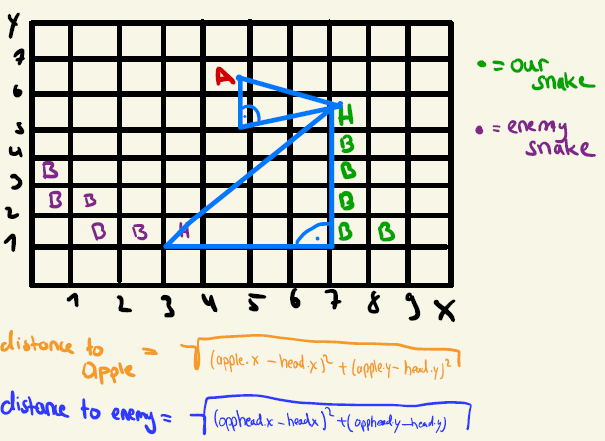
\includegraphics[scale=0.8]{calcs}
\caption{Calculations as graphical overview}
\end{figure}

\newpage
The code would look like this:
\begin{minted}{java}
//calculate the distance to other snake
double distanceToOtherSnake = 0;
   distanceToOtherSnake =  
   Math.sqrt(Math.pow((head.x - oppHead.x),2+Math.pow((head.yoppHead.y),2));
   System.out.println("Distance to other snake: " + distanceToOtherSnake);
\end{minted}
We need the distance to the other snakes head to decide whether our snake should dodge the opponents head or not. Because it only makes sense to dodge the opponent's head if it is one pixel away from our snakes head.\\
To handle the distances for each direction we used array lists. We basically calculate for each direction our snake possibly could take the  distance to the apple and to the other snakes head. You probably wonder why we should consider the distance to the enemy in this case. This is reasonable doubt but it is necessary for dodging the opponent's head. Because we take the directions which is the furthest distance to our opponent's head, to dodge his head.\\
\begin{minted}{java}
	ArrayList<Double> distancesToApple = new ArrayList<Double>();
        ArrayList<Double> distancesToOpp = new ArrayList<Double>();
        // mapping each direction of notLosing with the distance to the apple
        // and for distancesToOpp
        for (Direction dir: notLosing) {
                //calculate distances and put it in the arraylist
                int newHeadCoordinateX = snake.getHead().x + dir.dx;
                int newHeadCoordinateY = snake.getHead().y + dir.dy;
                double x = apple.x - newHeadCoordinateX;
                double y = apple.y - newHeadCoordinateY;
                double distance =Math.sqrt(Math.pow(x,2)+Math.pow(y,2));
                distancesToApple.add(distance);
                x = oppHead.x - newHeadCoordinateX;
                y = oppHead.y- newHeadCoordinateY;
                distance = Math.sqrt(Math.pow(x,2)+Math.pow(y,2));
                distancesToOpp.add((distance));
        }
\end{minted}
Now after knowing the distances our bot can look for the best directions. We are looping through our notLosing array and looking for min, max indexes of distances. So which direction is the one with the closest distance to the apple and the direction which is the furthest distance to the head of opponent.
\newpage
\begin{minted}{java}
	double max;
        double min;
        int indexOfMinDistance = 0;
        int indexOfMaxDistanceToOpp = 0;

        min = 0;
        max = 0;
        if(!distancesToApple.isEmpty())
            min = distancesToApple.get(0);
        if(!distancesToOpp.isEmpty())
            max = distancesToOpp.get(0);
         // choose the index of smallest distance
         // choose the index of furthest distance to opponents head
        if(min != 0 && max != 0) {
            for (int i = 1; i < notLosing.length; i++) {
                if (distancesToApple.get(i) < min) {
                    min = distancesToApple.get(i);
                    indexOfMinDistance = i;
                    // System.out.println(min);
                }
                if (distancesToOpp.get(i) > max) {
                    max = distancesToOpp.get(i);
                    indexOfMaxDistanceToOpp = i;
                }
            }
        }
\end{minted}
As last step our bot needs to decide which direction it should take based on the distance to the other snake and the possible directions of notLosing. If there is a possible direction which leads us not to die and where the distance to opponent snake's head is higher then 2 the bot takes the shortest path to the apple. If the distance to the opponents head is less or equal to 2, the bot dodges the head of the opponent. If none of these conditions met the bot just takes a valid move.
\begin{minted}{java}
	if(distancesToApple.size() > 0 && distanceToOtherSnake > 2){
            System.out.println("using shortest path");
            return notLosing[indexOfMinDistance];
        } else if ( distancesToOpp.size() > 0 && distanceToOtherSnake <= 2) {
            System.out.println("dodging opponents head");
           return  notLosing[indexOfMaxDistanceToOpp];
        } else{
            System.out.println("using valid moves");
            return validMoves[0];
        }
\end{minted}
After testing this bot and watching it for many games we noticed some problems, we also had in bots before. This bot's problem is, that it only calculates the next step. It would be more efficient to calculate more steps. With this current status the bot sometimes takes bads decisions. In some cases it takes the next closes direction to the apple and then it kills itself by hitting his own body. This is the problem of this greedy algorithm. 
\section{Experimental Results and Statistical Tests}
As in many areas of real world problem solving, deciding whether one case is better than another is not easy. In order to make a proper decision, analyzing statistical data is the best approach.\\
With insufficient data deciding if one bot is better than the other may lead to a wrong decision. This is comparable to the underlying principle of the Law of Large Numbers.\cite{LargeNumbers} For example, when you flip a coin the probability that heads or tails shows is for both 50\%(0.5). Now, flipping a coin ten times, if the result is 8 times heads and 2 times tails, we cannot conclude from this experiment that the probability of heads is 80\%(0.8) and of tails is 20\%(0.2). Doing the same experiment 1000 times will show that the average chance to hit heads or tails gets close to 50\%.
This is similar to our scenario. If we would let two bots play against each other for only five rounds and one snake is winning four times, it cannot be deduced that the winner is the better snake. So to determine whether a bot is better than another bot we decided to let them play against each other for thousand times and then compare the numbers of wins and loses. We also wanted to show statistically the average score, number of apples eaten and time played in each round. In the following section the results of our tests will be presented.\newpage
\subsection{Simulations}
First, the code of the "SnakesUIMain" class should be briefly remembered. The number of game rounds was set in the "start\_tournament\_n\_times" method and was set to five by default. To change the number of rounds we simply change the first parameter of the function.
\begin{minted}{Java}
start_tournament_n_times(5, bots);
\end{minted}
Changing the first parameter to thousand will lead to the game beeing started a thousand times. The framework uses .txt files to track the games. The folder structure, after setting the parameter to ten and letting the bots play, looks like this:
\begin{figure}[H]
    \centering
    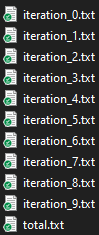
\includegraphics[scale=0.8]{logs_structure}
\caption{logstructure.png}
    \label{fig:logs_structure.png}
\end{figure}



The "iteration\_i.txt" file logs the data for each round. The "total.txt" file logs the summary of all rounds. The content of those files are structured in the following way:\\
\\
\begin{figure}[H]
    \centering
    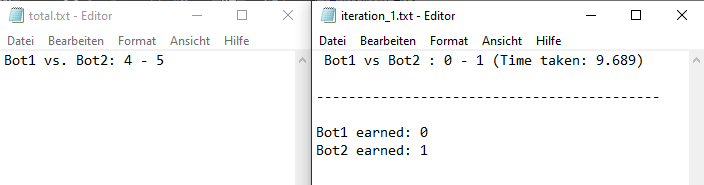
\includegraphics[scale=0.8]{logs_content}
\caption{logcontent.png}
    \label{fig:logs_content.png}
\end{figure}
For our statistical tests these information are not sufficient and not structured well, so we needed a new file structure. First of all, we had to think about what we really wanted to show and which variables were needed. We need variables like round ,results, apples eaten, time played. An example entry would look like:
\begin{itemize}
	\item 3,0,1,7,13,30.45
\end{itemize}
This would show the third round where the second bot has won. The first bot ate 7 and the second bot ate 13 apples. The round ended after 30.45 seconds.\\
We used as input 1000 games and collected a reasonable amount of data. 
\\The collect data contains the following scenarios:
\begin{itemize}
\item RecursiveBot vs. SimplifiedDijkstra
\item RecursiveBot vs. SimplifiedDijkstraV2
\end{itemize}
\subsection{Results of Different Algorithms}
The following table will show the measures of the 1000 games.\\
\subsubsection{RecursiveBot vs. SimplifiedDijkstra}
%--- Table  begin RecursiveBot vs SimplifiedDijkstra Results
\begin{table}[ht]
\caption{RecursiveBot vs SimplifiedDijkstra Results} % title of Table
\centering % used for centering table
\begin{tabular}{c c c c } % centered columns (4 columns)
\hline\hline %inserts double horizontal lines
Bot & avg. apples & max. apples & score\\ [0.5ex] % inserts table
%heading
\hline % inserts single horizontal line
RecursiveBot & 10 & 31 & 810 \\ % inserting body of the table
SimplifiedDijkstra & 7 & 26 & 184 \\
[1ex] % [1ex] adds vertical space
\hline %inserts single line
\end{tabular}
\label{table:recvsdijkstra} % is used to refer this table in the text
\end{table}
%--- Table end
This table shows clearly, that the recursive-bot\ref{Bot2} dominated the Simplified-Dijkstra bot. There is a huge difference in the score and a little difference in average apples eaten. This means that the recursive bot has the ability to eat many apples and to survive. However the other bot's max apple score is also notable.\\
Here are more interesting measures about the time taken for each round:\\
\begin{itemize}
	\item max. time: 137.53 s
	\item avg. time:  35.44 s
\end{itemize}
\subsubsection{RecursiveBot vs. SimplifiedDijkstraV2}

%--- Table  begin RecursiveBot vs SimplifiedDijkstra Results
\begin{table}[ht]
\caption{RecursiveBot vs SimplifiedDijkstraV2 Results} % title of Table
\centering % used for centering table
\begin{tabular}{c c c c } % centered columns (4 columns)
\hline\hline %inserts double horizontal lines
Bot & avg. apples & max. apples & score\\ [0.5ex] % inserts table
%heading
\hline % inserts single horizontal line
RecursiveBot & 8 & 32 & 650 \\ % inserting body of the table
SimplifiedDijkstraV2 & 6 & 20 & 297 \\
[1ex] % [1ex] adds vertical space
\hline %inserts single line
\end{tabular}
\label{table:recvsdijkstra2} % is used to refer this table in the text
\end{table}
%--- Table end
These results show that the Simplified-DijkstraV2 bot scored better than the previous version. But still had no chance to defeat the recursive-bot. It's interesting when comparing the two results. The difference of average apples eaten was 3 in the first test and in the second it dropped down to 2. Also the difference of max. apples was 5 before and then 12. But overall the second version performed better in manner of score.
If we look at the time taken for each round:\\
\begin{itemize}
	\item max. time: 107.07 s
	\item avg. time:  28.47 s
\end{itemize}
Looking at both results we can see that the time played is in the second test much shorter than in the first test.
\newpage
\subsubsection{Other Results}
%--- Table  begin other results
\begin{table}[H]
\caption{Other Results 1} % title of Table
\centering % used for centering table
\begin{tabular}{c c c c } % centered columns (4 columns)
\hline\hline %inserts double horizontal lines
total & RecursiveBot & SimplifiedDijkstra & $\Sigma$ \\ [0.5ex] % inserts table
%heading
\hline % inserts single horizontal line
apples & 10018 & 7340 & 17358 \\ % inserting body of the table
[1ex] % [1ex] adds vertical space
\hline %inserts single line
\end{tabular}
\label{table:otherresults1} % is used to refer this table in the text
\\Total time of 1000 rounds: 35442.56 seconds $=$ 590.7093 minutes $=$ 9.845155 Hours $=$ approx. 9 Hours 50 Minutes 42 seconds
\end{table}
%--- Table end

%--- Table  begin other results 2
\begin{table}[H]
\caption{Other Results 2} % title of Table
\centering % used for centering table
\begin{tabular}{c c c c } % centered columns (4 columns)
\hline\hline %inserts double horizontal lines
total & RecursiveBot &SimplifiedDijkstraV2 & $\Sigma$ \\ [0.5ex] % inserts table
%heading
\hline % inserts single horizontal line
apples & 8469 & 6055 & 14524 \\ % inserting body of the table
[1ex] % [1ex] adds vertical space
\hline %inserts single line
\end{tabular}
\label{table:otherresults2} % is used to refer this table in the text
\\Total time of 1000 rounds: 28465.49 seconds $=$ 474.4248 minutes $=$ 7.90708 Hours $=$ approx. 7 Hours 54 Minutes 25 seconds
\end{table}
%--- Table end
\newpage
\subsection{Charts}
\subsubsection{RecursiveBot vs. SimplifiedDijkstra}
%-- Score Bar Chart
\begin{figure}[H]
    \centering
    \includegraphics[scale=0.8]{{barchart1.png}}
    \caption{Barchart Wins}
    \label{fig:barchart1}
\end{figure}
%-- Time Boxplot
\begin{figure}[H]
    \centering
    \includegraphics[scale=0.8]{{boxplot1.png}}
    \caption{Boxplot of time played}
    \label{fig:boxplot1}
\end{figure}

\subsubsection{RecursiveBot vs. SimplifiedDijkstraV2}
%-- Score Bar Chart
\begin{figure}[H]
    \centering
    \includegraphics[scale=0.8]{{barchart2.png}}
    \caption{Barchart Wins}
    \label{fig:barchart1}
\end{figure}
%-- Time Boxplot
\begin{figure}[H]
    \centering
    \includegraphics[scale=0.8]{{boxplot2.png}}
    \caption{Boxplot of time played}
    \label{fig:boxplot1}
\end{figure}
\subsection{Evaluations}
In order to draw a conclusion from our statistical tests, we had to evaluate the diagrams. The boxplot clearly showed that the playing time of the competition between the RecursiveBot and the SimplifiedDijktra-Bot was on average longer than the other competition that was presented above. It was, however, not clear to us, how this information can be interpreted. One could say, that if bots are equally strong, the resulting playing time turns out to be longer, but the next chart clearly contradicted this statement.\\
\\ The maximum values of the playing time were also different. In the first competition, the maximum value was  137.53 seconds. In the second competition, the maximum value was only 107.07 seconds. We can thus state, that the playing time in the first test was significantly longer than in the second. \\
\\We interpreted the data in the following way: The first version of the Dijkstra is playing "safer" than the second one. But if we compare the wins and losses, we can make the assumption that the second one is more aggressive and either dies fast or takes out the opponent quickly. If we consider the maximum number of apples eaten, this interpretation gets emphasized, because the first version had only a maximum of 26  and the SimplifiedDijkstraV2 had a maximum of only 20 apples eaten.\\
\\Considering the statistical tests, it seemed that the recursive bot is the most promising one. The recursive bot tackled the problem of self-entrapment, which  seemed to be the biggest flaw of all other bots that we tested. 
In conclusion,  we can say, that the data analysis was able to give us new insights into the different strengths and weaknesses of our bots.  Statistical testing had the power to reveal the severity of certain flaws that our bots had. For example, without analyzing the data, it would have been impossible to state that the avoidance of self-entrapment is more important than finding the shortest path to the apple.  

\section{Conclusions and Future Work}
Since none of us had any previous knowledge about creating an intelligent bot, it was at the beginning very difficult for us to develop ideas that would be appropriate for our project and could also be handled by us. As already mentioned in chapter 3, we were able to meet weekly and in our meetings talked about different approaches and further improvements of our results. In this way, step by step, our ideas became more obvious and  manageable. Our way of working was to create several bots and have them compete against each other.  The statistical data of these competitions was subsequently analyzed, and then it was decided what had to be done next. From this data analysis, we were able to decide that the recursive bot \ref{RecursiveBot} was our best result. Analyzing the surroundings seems to be more important for a bot than finding the shortest distance to the apple and showing rudimentary evasive behavior towards the opponent.  
\subsection{How the team work went}

Since the project was very extensive and no team member had previously dealt with a comparable task, communication among the team members was essential. Creating solutions together or analyzing solutions together was necessary in order to identify weaknesses and work out strengths. The interactions between team members were always very friendly and solution oriented. Furthermore, different sections of the documentation and statistical analysis were evenly distributed among the team members so that everyone had roughly the same workload.\\
\\The size of the team was appropriate and also beneficial in two ways.  As each of us created bots, we always had enough bots to test against each other. With fewer team members, the number of bots would have also been fewer. Since there were only three of us, it was relatively easy to schedule meetings. If there had been more people involved, this would have been much more difficult. 

\subsection{What we learned}
When we were analyzing the statistical data, we realized that a simple assessment of a bot before any testing, aside from things like the time complexity, was not easily possible. Things that initially seemed very important turned out to be negligible. An example of this is the rudimentary evasive behavior of a bot concerning the opponent. Sound statements about bots could only be made after a game had been run several hundred or a thousand times. \\
\\We also discovered a successfull technique for detecting weaknesses of a bot. If you let a bot compete against itself, it is easy to determine what are its weaknesses by simple observing the movements of the snakes. Even in bots that turned out to be very successful, weaknesses could be found. In particular, our best result, RecursiveBot, could be further improved using this technique to identify its flaws. 
\\

\subsection{Ideas for the future development}
As already mentioned, the recursive bot turned out to be our strongest bot, so the obvious decision would be to use this bot as the basis for further development. The first thing that could be an important improvement is a structure that allows this bot to save ratings of squares of the game board. As already explained in chapter 6, the recursive bot uses a function that returns integer values that serve as a rating system for the surrounding squares. In its current version, the recursive bot calculates ratings for certain squares more than one time. This, of course, uses a lot of ressources that could be utilized for other things, like calculating positions of the opponent, which is our second idea for improving this bot. The current recursive bot does not calculate any future positions of the opponent. A second recursive structure could be implemented for this bot which does exactly that.\\
\\Another type of improvement would be the implementation of some form of advanced tactics. For example, the bot could try to actively trap the opponent. However, we currently do not know how this could be implemented.

\newpage
\bibliography{bibliography}
\bibliographystyle{plain}
\end{document}